\documentclass[12pt]{article}
\usepackage[letterpaper, margin=1in]{geometry}
\usepackage{amsmath}
\usepackage{amssymb}
\usepackage{listings}
\usepackage{enumitem}
\usepackage{parskip}
\usepackage{graphicx}
\usepackage{physics}
\newcommand{\Lagr}{\mathcal{L}}
\newcommand{\pderiv}[2]{\frac{\partial #1}{\partial #2}}
\newcommand{\vv}[2]{\vec{#1}_\text{#2}}
\newcommand{\powt}[2]{#1 \times 10^{#2}}

\newcommand{\xo}[0]{\hat{x}}
\newcommand{\po}[0]{\hat{p}}
\newcommand{\ad}[0]{a^\dagger}
\newcommand{\expect}[1]{\expectationvalue{#1}}

\title{The toilet water problem}
\author{Duncan Freeman}

\begin{document}
\maketitle
\section*{Introduction}
I rent a toilet which I suspect to have a leaky valve. This is evidenced by the fact that there is water condensating on the toilet's tank, which indicates that it's colder than its surroundings. It's cold to the touch as well.

But, I wondered, how much water is it losing? Is this worth worrying about?

I have recently purchased a thermal camera, so I decided to use some math and investigate this.

\begin{figure}
\begin{center}
    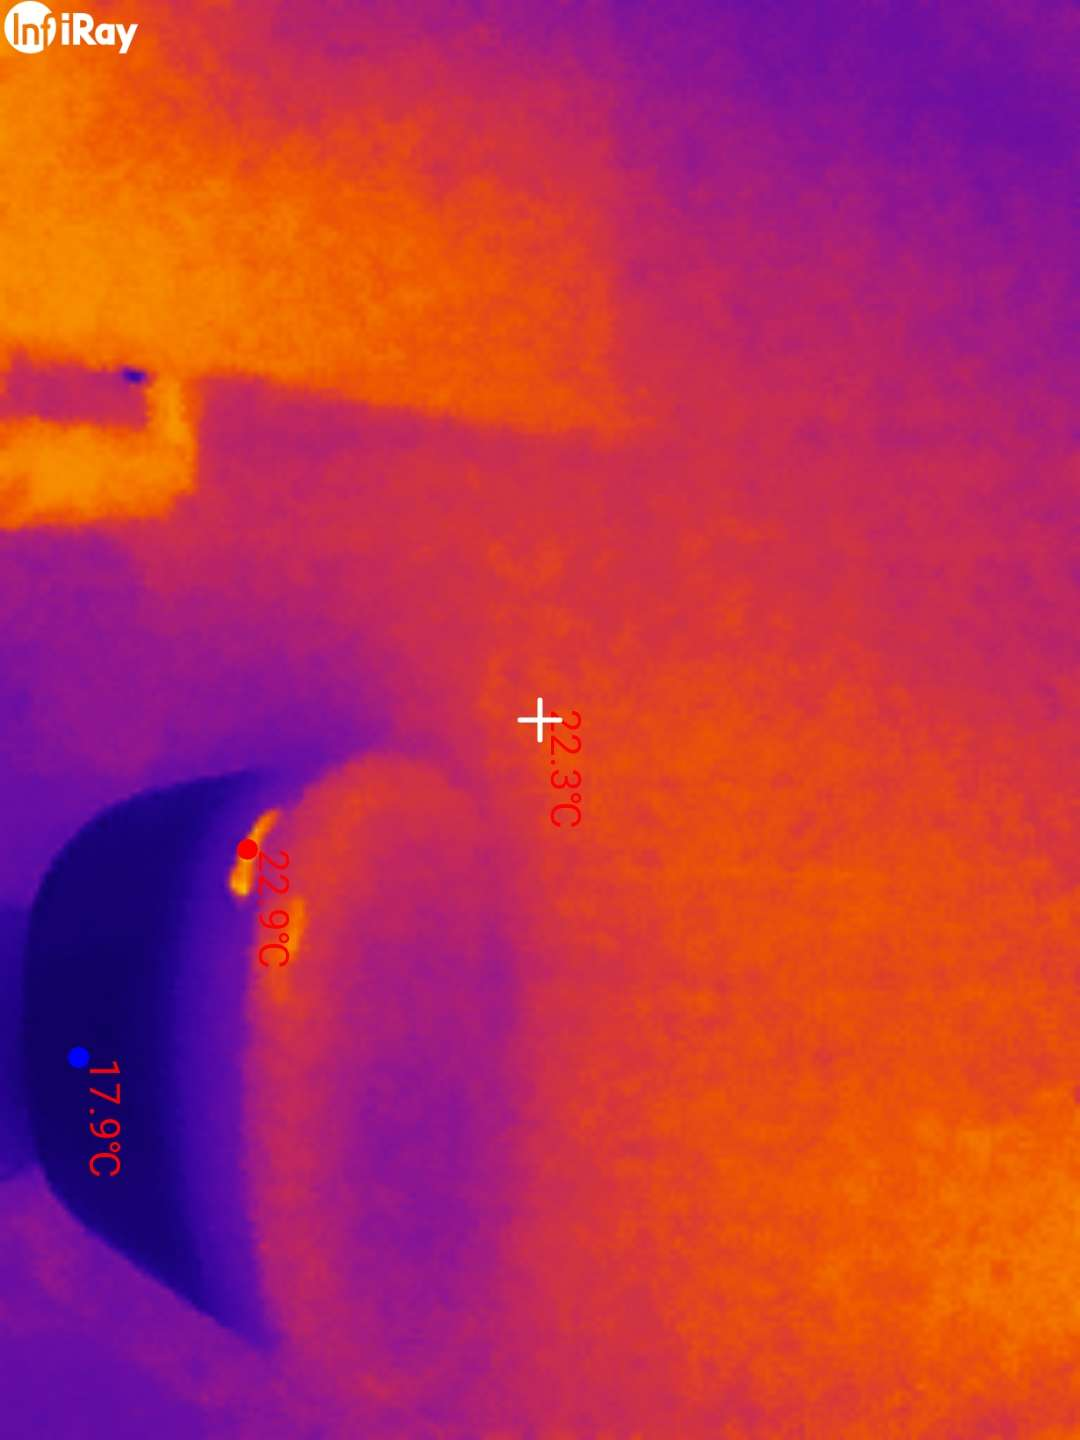
\includegraphics[angle=90,scale=0.2]{toilet_thermals.jpg}
    \caption{Thermal imaging of my lavatory. Note that the wall is roughly 22.3$^\circ$C, and the base of the toilet's tank (sitting against the wall) is 17.9$^\circ$C.}
    % NOTE: This is difficult to make out in the picture ...
\end{center}
\end{figure}

\begin{figure}
\begin{center}
    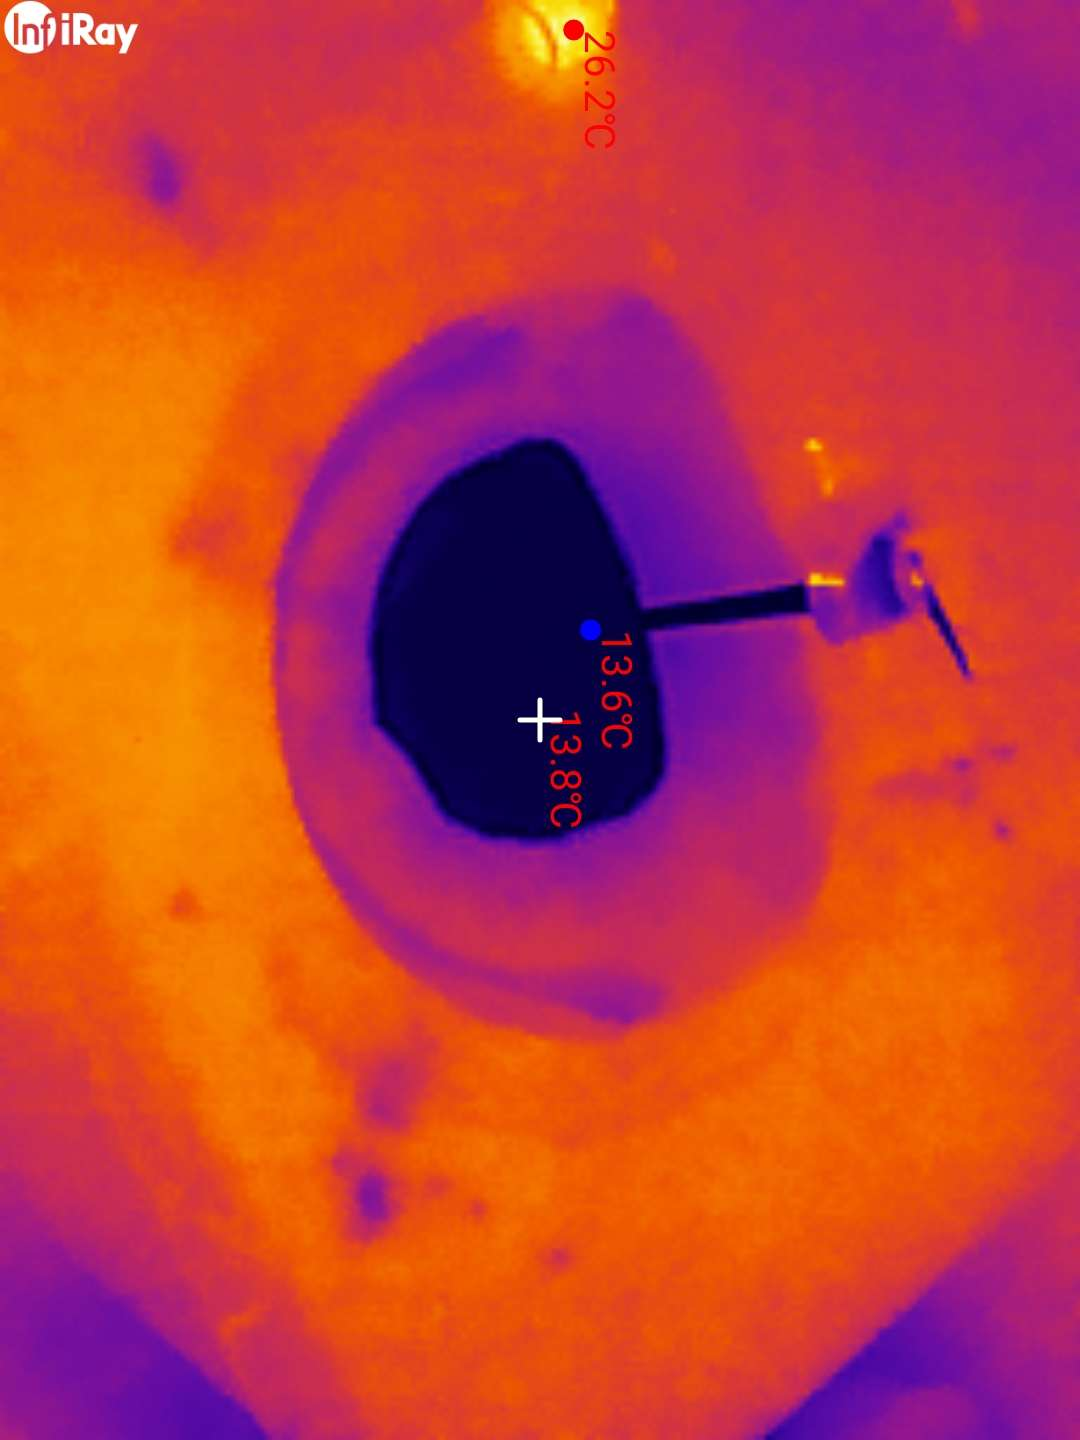
\includegraphics[angle=90,scale=0.2]{source_water_thermals.jpg}
    \caption{Thermal imaging of running water in my sink. This is to get an idea of the temperature of the water in the pipes. It's about 13.6$^\circ$C at the coldest, right from the tap.}
    % NOTE: This is difficult to make out in the picture ...
\end{center}
\end{figure}

\section*{Coefficients}
The tank lists itself as 6 Liters per flush; I flushed the toilet and it seemed to have an extra $10\%$ or so left at the very bottom of the tank during the lowest point of the flush. So $V \approx 6.6 L$.

I used the thermal camera to take temperature readings of the toilet's tank and its surroundings. I also took a temperature reading of the water coming in from the rest of the piping.

To summarize, here is a table of coefficients and their values:

\begin{center}
\begin{tabular}{ | c | c | l | }
    \hline
    Coefficient & Value & Description \\
    \hline
    \hline
    % $T_E$ & 22.3$^\circ$C & Temperature of the environment \\
    % \hline
    $T_O$ & 17.0$^\circ$C & Equilibrium temperature outside the tank \\
    \hline
    $T_I$ & 16.6$^\circ$C & Equilibrium temperature inside the tank \\
    \hline
    $T_W$ & 13.6$^\circ$C & Temperature of the incoming water \\
    \hline
    $V$ & 6.6 L & Volume of the tank \\
    \hline
    $k$ & 0.92 $W/(m^{\circ}K)$ & Approximate thermal conductivity (concrete) \\
    \hline
    $\Delta x$ & 0.01 m & Approximate thickness of the tank walls \\
    \hline
    $C_s$ & 4.184 $kJ/(L^{\circ}C)$ & Specific heat of water \\
    \hline
\end{tabular}
\end{center}

We are interested in calculating the flow rate $f$, measured in Liters/hour indicating how much water we are losing.

\clearpage
\section*{Solving the problem}
We'll assume the water is well mixed, so that the equilibrium temperature at the point measured is representative. 

%We'll also assume that the temperature measured on the surface of the tank is indicative of the temperature on the inside.

Let's assume that the change in energy due to the outflow of warmed up tank water (and subsequent inflow of cold water) is equal to the difference in temperature between the environment and the tank walls. 
\[ \Delta Q = 0 = \pderiv{Q_\text{in}}{t} - \pderiv{Q_\text{out}}{t} \]

\section*{Energy lost per unit time}
Let's calculate the change in energy due to outflow:
\[ \pderiv{Q_\text{out}}{t} = \left(\pderiv{V}{t} \cdot \frac{m}{V}\right) C_s \Delta T_\text{water} = f C_s (T_w - T_I) \]

\section*{Energy gained per unit time}
Now let's form the other side the the equation, which denotes the instantaneous temperature gained from the environment per unit time. 

Conductance is given by:
\[ U = \frac{k}{\Delta x} \]

We'll approximate the tank as a sphere. So, if its volume is 6.6L then its area must be:
\[ A = 4\pi r^2 \]
\[ V = \tfrac{4}{3}\pi r^3 \]
\[ A = 4\pi(V \cdot \tfrac{3}{4\pi})^{2/3} \approx 0.17 \text{ m}^2 \]

Now we apply Fourier's law:
\[ \pderiv{Q_\text{out}}{t} = UA(-\Delta T) = UA(T_O - T_I) \]

\section*{Solving for $f$}
\[ f C_s (T_w - T_I) = \frac{k}{\Delta x} A (T_O - T_I) \]
\[ f = \frac{Ak (T_O - T_I)}{C_s \Delta x (T_w - T_I)} \approx 1.79 \tfrac{L}{hr} \]



%\[ \Delta T_2 = \pderiv{T_2}{t} = \Delta T_\text{env $\to$ tank} = T_E - T_O \]


%We can now solve for an (approximate) flow rate:
%\[ \Delta T_1 = -\Delta T_2 \]

%\[ f\cdot\frac{T_w - T_I}{V} = T_O - T_E \]
%\[ f = \frac{V(T_O - T_E)}{T_w - T_I} \]

\end{document}

